\section{Observations}
\label{sec:obs}
\begin{itemize}
  \item Parent sample: LoVoCCS, selected at $0.03 < z < 0.12$ and
        $L_{{\rm X},500c}>10^{44}$\,erg\,s$^{-1}$ in the 0.1--2.4\,keV
        band \citep{Fu2024}. The working target list contains 107 named
        clusters; the radio and archival X-ray subsets below do not inherit
        the parent survey's completeness.
  \item Radio: 26 targets with usable LoTSS DR3 144\,MHz images
        \citep{Shimwell2026}, $z=0.0353$--$0.1198$. The adopted inputs are
        3\,Mpc squares on a $128\times128$ grid, extracted from 80$'$
        cutouts centred on catalogue coordinates; the 1\,Mpc comparison
        has 25 targets (A1750 is absent). Images are transformed as
        ${\rm arcsinh}(S/\sigma_{\rm rms})$, using a sigma-clipped rms
        measured on each resampled cutout before masking (median
        0.143\,mJy\,beam$^{-1}$ for the 3\,Mpc sample).
  \item Native restoring beams: 22 cutouts have 9$''$ FWHM, while A2147,
        A2443, A2589 and A2703 have 6$''$ FWHM. The current processing
        assumes 9$''$ for the masking and mock beam and does not homogenise
        the observed beams. \todo{Resolve or quantify this beam mismatch
        before claiming matched radio resolution.}
  \item Compact-source masking: detect connected islands above
        $5\sigma_{\rm rms}$; mask those whose area above half their peak is
        at most ten assumed beam half-power areas. Replace each masked
        disc with the surrounding annular median plus Gaussian noise at
        the measured rms. The same procedure is applied to field-injected
        mocks. This is a morphological compact-source filter, not an
        identification or complete subtraction of AGN emission.
  \item Chandra archive used here: 55 public observations of 19 radio
        targets (25 ACIS-I and 30 ACIS-S observations). The processed
        sample uses the 25 ACIS-I observations of 15 targets; ACIS-S
        requires a separate response/footprint treatment. The
        Cycle-22-equivalent target exposures span 6.2--229.4\,ks,
        with median 31.3\,ks; these are not raw archival exposure times.
  \item X-ray processing: 0.1--2\,keV events, CIAO exposure maps at
        1.2\,keV, and particle background estimated from 9.5--12\,keV
        events. Subtract the estimated particle counts before dividing by
        the Cycle-22-equivalent exposure, then restore the reference mock
        particle level. Fill chip gaps by local interpolation and apply
        the common ${\rm arcsinh}(R/a)$ stretch. This effective-area
        correction is a monochromatic approximation; the count model and
        remaining footprint limitations are in Section~\ref{sec:xray}.
  \item Geometry: X-ray images are centred on the smoothed X-ray peak
        within 2$'$ of the catalogue position, unlike the radio cutouts.
        The X-ray grid has 128 pixels per side at approximately
        18.9\,kpc per pixel; pixels outside the common circular aperture
        are zero. Its radius is approximately 485\,kpc for $z\geq0.05$
        and decreases with angular-diameter distance below that redshift
        (an 8$'$ radius). The two bands are not registered to a common
        physical centre.
  \item Weak-lensing masses: 18 of the 26 radio targets, including 11 of
        the 15 ACIS-I targets. Use the LoVoCCS processing outputs'
        single-peak NFW $M_{200c}$ fits, converted to $M_{500c}$ with the
        fit's own concentration relation and cosmology; carry the bootstrap
        interval endpoints through the same conversion. The median
        fractional uncertainty on the input $M_{200c}$ is 23 per cent.
        The older 1\,Mpc radio subset has 17 masses among 25 targets.
  \item Observations supply the inference sample and unlabelled
        forward-model comparisons/calibration; they have no independent
        pseudo-TSC labels. Radio--X-ray agreement is a consistency check.
        The optical-structure experiment in Section~\ref{sec:results}
        uses idealised simulated inputs, not observed member catalogues.
        \todo{Add a target table with coordinates, redshift, radio beam
        and rms, Chandra ObsIDs and equivalent exposure, and weak-lensing
        mass with uncertainty.}
\end{itemize}
\begin{figure*}
  \centering
  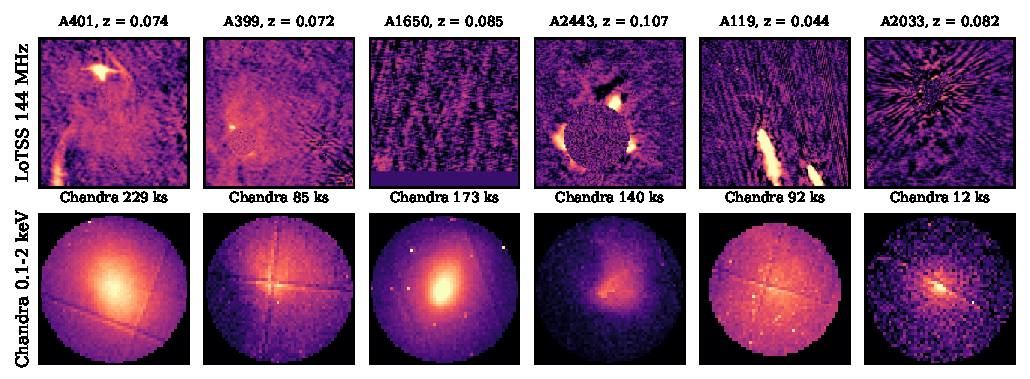
\includegraphics[width=\textwidth]{fig_obs_gallery.pdf}
  \caption{Six LoVoCCS targets with both LoTSS DR3 and Chandra ACIS-I
  data, displayed over approximately 1\,Mpc about each band's adopted
  centre. These panels show the 1\,Mpc radio comparison inputs and central
  crops of the X-ray inputs; the adopted radio-only analysis uses 3\,Mpc
  cutouts. Top:
  ${\rm arcsinh}(S/\sigma_{\rm rms})$ at 144\,MHz, with compact sources
  masked (the noise-filled discs). Bottom: ${\rm arcsinh}(R/a)$ for the
  processed 0.1--2\,keV count rate, normalised by the
  Cycle-22-equivalent exposure (given above each panel), with particle
  background correction, the reference particle level restored, and chip
  gaps filled; pixels outside the common aperture are zero.}
  \label{fig:obs_examples}
\end{figure*}
